\documentclass[aspectratio=169,11pt]{beamer}

% ---------------- Packages ----------------
\usepackage[utf8]{inputenc}
\usepackage[T1]{fontenc}
\usepackage{xcolor}
\usepackage{booktabs}
\usepackage{amsmath,amssymb}
\usepackage{hyperref}
\usepackage{graphicx}
\usepackage{tikz}
\usetikzlibrary{positioning,arrows.meta,calc}

\graphicspath{{../}{./}}

\IfFileExists{opensans.sty}{\usepackage[default,scale=0.95]{opensans}}{}

% ---------------- Theme ----------------
\definecolor{amritaMaroon}{HTML}{A4123F}

\usetheme{Madrid}
\usecolortheme[named=amritaMaroon]{structure}
\setbeamertemplate{navigation symbols}{}
\setbeamertemplate{footline}[frame number]

\begin{document}

%%%%%%%%%%%%%%%%%%%%%%%%%%%%%%%%%%%%%%%%%%%%%%%%%%%%%
%%%%%%%%%%%%%%%%%%%% TITLE PAGE %%%%%%%%%%%%%%%%%%%%%
%%%%%%%%%%%%%%%%%%%%%%%%%%%%%%%%%%%%%%%%%%%%%%%%%%%%%

\begin{frame}

\begin{tikzpicture}[remember picture,overlay]
\node[
fill=amritaMaroon,
text=white,
font=\bfseries\scriptsize,
anchor=north east,
rounded corners=2pt,
inner sep=4pt]
at ($(current page.north east)+(-0.3,-0.3)$)
{Type 2: Application Project};
\end{tikzpicture}

\centering

\includegraphics[height=1.45cm,keepaspectratio]{logo.png}

\vspace{0.12cm}

{\large\bfseries\textcolor{amritaMaroon}{Cycle-Aware Graph Learning for Coordinated\\[2pt] Anti-Money Laundering Detection}}\par

\vspace{0.10cm}

{\scriptsize
Enhancing GraphSAGE using Random Walk Cycle Features and Structural Edge Attention\par
}

\vspace{0.15cm}

{\scriptsize
\textbf{23CSE498 -- Project Phase}
\hspace{0.5cm}|\hspace{0.5cm}
\textbf{Team Number : [XX]}\par
}

\vspace{0.22cm}

\begin{columns}[c]
\column{0.53\textwidth}
\centering
\scriptsize
\renewcommand{\arraystretch}{1.08}
\begin{tabular}{|c|c|l|}
\hline
\textbf{S.No} & \textbf{Register Number} & \textbf{Student Name}\\
\hline
1 & & \\
\hline
2 & & \\
\hline
3 & & \\
\hline
4 & & \\
\hline
\end{tabular}

\column{0.47\textwidth}
\centering
\scriptsize
Guide:\\[1pt]
\textbf{Dr. Anbazhagan M}\\[4pt]
Department of Computer Science and Engineering\\[5pt]
\today
\end{columns}

\end{frame}

%%%%%%%%%%%%%%%%%%%%%%%%%%%%%%%%%%%%%%%%%%%%%%%%%%%%%
%%%%%%%%%%%%%%%%%%%% SLIDE 2 %%%%%%%%%%%%%%%%%%%%%%%%
%%%%%%%%%%%%%%%%%%%%%%%%%%%%%%%%%%%%%%%%%%%%%%%%%%%%%

\section{Phase 3A}

\begin{frame}{1. Phase 3A: Random Walk Cycle Feature Extractor}

\framesubtitle{Novel Feature Engineering}

\begin{columns}[T]

%%%%%%%%%%%%%%%%%%%%%%%%%%%%%%%%%%%%%%%%%%%%%%%
\column{0.58\textwidth}

{\footnotesize
\textbf{Objective}

Detect hidden circular money laundering patterns by extracting structural cycle-aware features before Graph Neural Network training.

\vspace{0.15cm}

\textbf{Methodology}

\begin{itemize}\setlength{\itemsep}{2.5pt}\setlength{\parskip}{0pt}

\item Construct the transition probability matrix
$P = D_{\mathrm{out}}^{-1} A$.

\item Compute random walk return probabilities
$P^2, P^3, P^4, P^5$.

\item Generate eight cycle-aware edge features.

\item Expand edge features from \textbf{14 to 22}.

\item Maintain zero temporal leakage using only the training topology.

\end{itemize}
}

%%%%%%%%%%%%%%%%%%%%%%%%%%%%%%%%%%%%%%%%%%%%%%%
\column{0.42\textwidth}

\centering

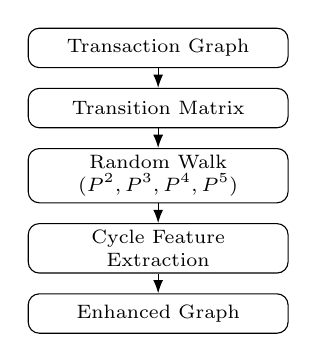
\begin{tikzpicture}[
node distance=0.25cm,
every node/.style={
draw,
rounded corners,
minimum width=3.3cm,
minimum height=0.50cm,
align=center,
font=\scriptsize,
inner sep=2.5pt}
]

\node (a){Transaction Graph};
\node[below=of a](b){Transition Matrix};
\node[below=of b](c){Random Walk\\($P^2,P^3,P^4,P^5$)};
\node[below=of c](d){Cycle Feature\\Extraction};
\node[below=of d](e){Enhanced Graph};

\draw[-{Latex}] (a)--(b);
\draw[-{Latex}] (b)--(c);
\draw[-{Latex}] (c)--(d);
\draw[-{Latex}] (d)--(e);

\end{tikzpicture}

\end{columns}

\vspace{0.18cm}

{\footnotesize
\textbf{Outcome}

Cycle-aware structural information enables the model to identify hidden laundering cycles that cannot be captured using traditional transaction features alone.
}

\end{frame}

%%%%%%%%%%%%%%%%%%%%%%%%%%%%%%%%%%%%%%%%%%%%%%%%%%%%%
%%%%%%%%%%%%%%%%%%%% SLIDE 3 %%%%%%%%%%%%%%%%%%%%%%%%
%%%%%%%%%%%%%%%%%%%%%%%%%%%%%%%%%%%%%%%%%%%%%%%%%%%%%

\section{Phase 3B}

\begin{frame}{2. Phase 3B: Cycle-Aware Attention Layer}

\framesubtitle{Graph Neural Network Enhancement}

\begin{columns}[T]

%%%%%%%%%%%%%%%%%%%%%%%%%%%%%%%%%%%%%%%%%%%%%%%
\column{0.48\textwidth}

{\footnotesize
\textbf{Objective}

Improve GraphSAGE by allowing the model to focus on suspicious transaction paths instead of treating every neighboring transaction equally.

\vspace{0.15cm}

\textbf{Limitation of Vanilla GraphSAGE}

\begin{itemize}\setlength{\itemsep}{1.5pt}\setlength{\parskip}{0pt}

\item Uses mean aggregation to combine neighbor information.

\item Every transaction contributes equally.

\item Suspicious laundering transactions are diluted by many normal transactions.

\item Hidden circular money laundering patterns become difficult to detect.

\end{itemize}
}

%%%%%%%%%%%%%%%%%%%%%%%%%%%%%%%%%%%%%%%%%%%%%%%
\column{0.52\textwidth}

\centering

\renewcommand{\arraystretch}{1.08}
\scriptsize

\begin{tabular}{|p{2.6cm}|p{2.6cm}|}
\hline
\textbf{Vanilla GraphSAGE} & \textbf{Proposed Model} \\
\hline
Mean Aggregation & Attention Aggregation \\
\hline
Equal Importance & Weighted Importance \\
\hline
Signal Dilution & Focus on Cycle Paths \\
\hline
Lower Detection Accuracy & Higher Detection Accuracy \\
\hline
\end{tabular}

\vspace{0.18cm}
\raggedright
{\footnotesize
\textbf{Proposed Solution}

Introduce a Cycle-Aware Attention Layer that assigns larger attention weights to transactions having stronger cycle probabilities.
}

\end{columns}

\vspace{0.15cm}

{\footnotesize
\textbf{Outcome}

The attention mechanism preserves important cycle information and improves message passing for coordinated money laundering detection.
}

\end{frame}

%%%%%%%%%%%%%%%%%%%%%%%%%%%%%%%%%%%%%%%%%%%%%%%%%%%%%
%%%%%%%%%%%%%%%%%%%% SLIDE 4 %%%%%%%%%%%%%%%%%%%%%%%%
%%%%%%%%%%%%%%%%%%%%%%%%%%%%%%%%%%%%%%%%%%%%%%%%%%%%%

\section{Phase 3C}

\begin{frame}{3. Phase 3C: Scientific Ablation Study}

\framesubtitle{Experimental Validation}

{\footnotesize
\textbf{Objective}

Evaluate the contribution of each proposed component using identical training and testing conditions.
}

\vspace{0.15cm}

\begin{columns}[T]

%%%%%%%%%%%%%%%%%%%%%%%%%%%%%%%%%%%%%%%%%%%%%%%
\column{0.52\textwidth}

{\footnotesize\textbf{Experimental Configurations}}\par
\vspace{0.06cm}
\centering
\setlength{\tabcolsep}{3pt}
\renewcommand{\arraystretch}{1.05}
\scriptsize

\begin{tabular}{|l|c|c|}
\hline
\textbf{Model} & \textbf{Cycle Features} & \textbf{Attention} \\
\hline
Vanilla GraphSAGE & No & No \\
\hline
GraphSAGE + Cycle Features & Yes & No \\
\hline
Proposed Model & Yes & Yes \\
\hline
\end{tabular}

\vspace{0.2cm}
\raggedright
{\footnotesize\textbf{Performance Comparison}}\par
\vspace{0.06cm}
\centering
\setlength{\tabcolsep}{3pt}
\renewcommand{\arraystretch}{1.05}
\scriptsize

\begin{tabular}{|l|c|c|}
\hline
\textbf{Model} & \textbf{PR-AUC} & \textbf{Complete Ring Recall} \\
\hline
Vanilla GraphSAGE & 0.3235 & 76.9\% \\
\hline
+ Cycle Features & 0.1113 & 63.8\% \\
\hline
+ Cycle Attention & \textbf{0.5759} & \textbf{85.2\%} \\
\hline
\end{tabular}

%%%%%%%%%%%%%%%%%%%%%%%%%%%%%%%%%%%%%%%%%%%%%%%
\column{0.48\textwidth}

\raggedright
{\footnotesize
\textbf{Key Findings}

\vspace{0.06cm}

\begin{itemize}\setlength{\itemsep}{5pt}\setlength{\parskip}{0pt}

\item Cycle features alone reduced performance due to mean aggregation.

\item Cycle-Aware Attention effectively preserved structural information.

\item The proposed model achieved a \textbf{78\% improvement in PR-AUC} and significantly improved complete laundering ring detection.

\end{itemize}
}

\end{columns}

\end{frame}

%%%%%%%%%%%%%%%%%%%%%%%%%%%%%%%%%%%%%%%%%%%%%%%%%%%%%
%%%%%%%%%%%%%%%%%%%% SLIDE 5 %%%%%%%%%%%%%%%%%%%%%%%%
%%%%%%%%%%%%%%%%%%%%%%%%%%%%%%%%%%%%%%%%%%%%%%%%%%%%%

\section{Experimental Results}

\begin{frame}{4. Experimental Results}

\framesubtitle{Performance Evaluation of the Proposed Model}

\begin{columns}[T]

%%%%%%%%%%%%%%%%%%%%%%%%%%%%%%%%%%%%%
\column{0.48\textwidth}

{\footnotesize
\textbf{Performance Improvements}

\begin{itemize}\setlength{\itemsep}{3.5pt}\setlength{\parskip}{0pt}

\item Precision-Recall AUC\\[1pt]
$0.3235 \rightarrow 0.5759$

\item Relative Improvement\\[1pt]
$+78\%$

\item Complete Ring Recall\\[1pt]
$76.9\% \rightarrow 85.2\%$

\item Mean Pattern Coverage\\[1pt]
$95.2\%$

\end{itemize}
}

%%%%%%%%%%%%%%%%%%%%%%%%%%%%%%%%%%%%%
\column{0.52\textwidth}

\centering

\renewcommand{\arraystretch}{1.12}
\small

\begin{tabular}{lcc}
\toprule
Metric & Baseline & Proposed\\
\midrule
PR-AUC & 0.3235 & \textbf{0.5759}\\
Ring Recall & 76.9\% & \textbf{85.2\%}\\
Alert Recall & 98.7\% & 98.7\%\\
Mean Coverage & 89.6\% & \textbf{95.2\%}\\
\bottomrule
\end{tabular}

\end{columns}

\vspace{0.18cm}

{\footnotesize
\textbf{Observation}

The proposed Cycle-Aware GraphSAGE significantly improves the identification of coordinated laundering rings while maintaining high alert recall.
}

\end{frame}

%%%%%%%%%%%%%%%%%%%%%%%%%%%%%%%%%%%%%%%%%%%%%%%%%%%%%
%%%%%%%%%%%%%%%%%%%% SLIDE 6 %%%%%%%%%%%%%%%%%%%%%%%%
%%%%%%%%%%%%%%%%%%%%%%%%%%%%%%%%%%%%%%%%%%%%%%%%%%%%%

\section{Pattern Level Evaluation}

\begin{frame}{5. Pattern-Level Performance}

\framesubtitle{Evaluation Across Different Laundering Patterns}

\centering

\renewcommand{\arraystretch}{1.15}
\small

\begin{tabular}{lcccc}
\toprule
Pattern & Any & Majority & Full & Coverage\\
\midrule
Cycle & 96.4\% & 96.4\% & 85.7\% & 93.9\%\\
Fan-Out & 100.0\% & 96.4\% & 92.9\% & 96.4\%\\
Gather-Scatter & 100.0\% & 100.0\% & 81.4\% & 96.1\%\\
\midrule
Overall & 98.7\% & 98.3\% & 85.2\% & 95.2\%\\
\bottomrule
\end{tabular}

\vspace{0.3cm}

\raggedright
{\footnotesize
\textbf{Discussion}

\begin{itemize}\setlength{\itemsep}{3pt}\setlength{\parskip}{0pt}

\item Pattern-level evaluation measures how well the model detects entire laundering networks rather than individual suspicious transactions.

\item The proposed model achieves high detection accuracy across multiple money laundering typologies.

\end{itemize}
}

\end{frame}

%%%%%%%%%%%%%%%%%%%%%%%%%%%%%%%%%%%%%%%%%%%%%%%%%%%%%
%%%%%%%%%%%%%%%%%%%% SLIDE 7 %%%%%%%%%%%%%%%%%%%%%%%%
%%%%%%%%%%%%%%%%%%%%%%%%%%%%%%%%%%%%%%%%%%%%%%%%%%%%%

\section{Conclusion}

\begin{frame}{6. Conclusion}

\framesubtitle{Summary of the Proposed Framework}

{\footnotesize
\textbf{Major Contributions}

\vspace{0.15cm}

\begin{enumerate}\setlength{\itemsep}{3pt}\setlength{\parskip}{0pt}

\item Developed a Random Walk Cycle Feature Extractor to capture hidden circular transaction behaviour.

\item Introduced a Cycle-Aware Attention Layer that prioritizes suspicious transaction paths during message passing.

\item Validated the contribution of each component using a Scientific Ablation Study.

\item Improved coordinated Anti-Money Laundering detection over Vanilla GraphSAGE.

\end{enumerate}

\vspace{0.25cm}

\begin{block}{Final Outcome}
The proposed Cycle-Aware Graph Learning framework combines structural cycle features and attention-based message passing to significantly improve the detection of coordinated money laundering activities.
\end{block}
}

\end{frame}

%%%%%%%%%%%%%%%%%%%%%%%%%%%%%%%%%%%%%%%%%%%%%%%%%%%%%
%%%%%%%%%%%%%%%%%%%% THANK YOU %%%%%%%%%%%%%%%%%%%%%%
%%%%%%%%%%%%%%%%%%%%%%%%%%%%%%%%%%%%%%%%%%%%%%%%%%%%%

\begin{frame}

\centering

\vspace{1.5cm}

{\Huge\textbf{\textcolor{amritaMaroon}{Thank You}}}

\vspace{0.5cm}

{\Large Questions?}

\end{frame}

\end{document}